\section{Global Qt functions and macros}
Qt has its functionality separated into modules\index{module}. There is one special module (incarnated in QtCore module) called QtGlobal\index{QtGlobal}. QtGlobal is contained within single header file\fdocinlinecode{text}{!}{qglobal.h}. QtGlobal contains following:
\begin{itemize}
\item
type clones (\autoref{table:types}) for every standard \cpp type

\item
functions

\item
macros\index{macro}
\end{itemize}

\begin{table}[ht]
\begin{center}
\caption{Qt Creator minimal plugins setup on x86 architecture (Linux)}\label{table:types}
\begin{tabular}{c | c}
orignal type name & Qt type name \\
\hline
\fdocinlinecode{cpp}{!}{signed char} & \fdocinlinecode{cpp}{!}{qint8} \\ 
\fdocinlinecode{cpp}{!}{unsigned char} & \fdocinlinecode{cpp}{!}{quint8} \\ 
\fdocinlinecode{cpp}{!}{short} & \fdocinlinecode{cpp}{!}{qint16} \\ 
\fdocinlinecode{cpp}{!}{unsigned short} & \fdocinlinecode{cpp}{!}{quint16} \\ 
\fdocinlinecode{cpp}{!}{int} & \fdocinlinecode{cpp}{!}{qint32} \\ 
\fdocinlinecode{cpp}{!}{unsigned int} & \fdocinlinecode{cpp}{!}{quint32} \\ 
\fdocinlinecode{cpp}{!}{qint64} & \fdocinlinecode{cpp}{!}{qlonglong} \\ 
\fdocinlinecode{cpp}{!}{quint64} & \fdocinlinecode{cpp}{!}{qulonglong} \\ 
\fdocinlinecode{cpp}{!}{unsigned char} & \fdocinlinecode{cpp}{!}{uchar} \\ 
\fdocinlinecode{cpp}{!}{unsigned short} & \fdocinlinecode{cpp}{!}{ushort} \\ 
\fdocinlinecode{cpp}{!}{unsigned int} & \fdocinlinecode{cpp}{!}{uint} \\ 
\fdocinlinecode{cpp}{!}{unsigned long} & \fdocinlinecode{cpp}{!}{ulong} \\
\fdocinlinecode{cpp}{!}{double} & \fdocinlinecode{cpp}{!}{qreal}
\end{tabular}
\end{center}
\end{table}

\subsection{Fundamental functions}
QtGlobal offers very fundamental functions for value-based comparing and other basic tasks. These functions (often) wrap similar functions from standard C/\cpp library\index{standard library}. Most used functions are:
\begin{description}
\item[T qAbs(const T \& value)] \hfill \\
Returns absolute value of input parameter.
\item[const T \& qBound(const T \& min, const T \& value, const T \& max)] \hfill \\
Returns input value \enquote{rounded} to fit within bounds.
\item[double qInf()] \hfill \\
Returns value which represents infinity.
\item[qint64 qRound64(qreal value) and int qRound(qreal value)] \hfill \\
Mathematically rounds input paramater either to 64/32 bit integer.
\end{description}

All functons can be found in\fdocinlinecode{text}{!}{/qt-root-directory/include/QtCore/qglobal.h}.

\subsection{Producing console outputs with QDebug class}
Qt offers better way to produce console\index{console} printing for debugging purposes via \fdocinlinecode{cpp}{!}{QDebug}\index{\fdocinlinecode{cpp}{!}{QDebug}} class and\fdocinlinecode{cpp}{!}{QtMessageHandler qInstallMessageHandler(QtMessageHandler handler} function. You can always use traditional\fdocinlinecode{cpp}{!}{std::cout} for console printing but\fdocinlinecode{cpp}{!}{QDebug} way is much better.

Basic syntax for using\fdocinlinecode{cpp}{!}{QDebug} is fairly simple (\autoref{listing:qdebug}).

\begin{fdoccode}{cpp}{listing:qdebug}{Basic QDebug usage}
qDebug() << "Print this to standard output.";
qDebug("Print number %d.\n", 10);
\end{fdoccode}

First\fdocinlinecode{cpp}{!}{qDebug()} usage requires explicit\fdocinlinecode{cpp}{!}{<QDebug>} inclusion because operator\fdocinlinecode{cpp}{!}{<<} is used. Second usage acts as wrapper for the\fdocinlinecode{cpp}{!}{printf()} function from standard C library. You can use also\fdocinlinecode{cpp}{!}{qWarning()},\fdocinlinecode{cpp}{!}{qCritical()} and\fdocinlinecode{cpp}{!}{qFatal()} in accordance to importance of message. Default implementation halts an application if\fdocinlinecode{cpp}{!}{qFatal()} is called.

You can implement custom behavior for previous functions very simply:
\begin{enumerate}
\item
You need to implement global (or static) function with signature\fdocinlinecode{cpp}{!}{void (*function)(QtMsgType, const QMessageLogContext &, const QString &)}. Typical\\ implementation may look like \autoref{listing:qdebug2}.

\item
You need to assign handler to this function via\fdocinlinecode{cpp}{!}{qInstallMessageHandler()} function.
\end{enumerate}

\begin{fdoccode}{cpp}{listing:qdebug2}{Typical printing handler for QDebug}
void debug_handler(QtMsgType type, const QMessageLogContext &placement, const QString &message) {
    switch (type) {
	case QtDebugMsg:
	    fprintf(stderr, "[%s] INFO (%s, line %d) : %s\n",
		    APP_LOW_NAME,
		    placement.file,
		    placement.line,
		    qPrintable(message));
	    break;
	case QtWarningMsg:
	    fprintf(stderr, "[%s] WARNING (%s, line %d) : %s\n",
		    APP_LOW_NAME,
		    placement.file,
		    placement.line,
		    qPrintable(message));
	    break;
	case QtCriticalMsg:
	    fprintf(stderr, "[%s] CRITICAL (%s, line %d) : %s\n",
		    APP_LOW_NAME,
		    placement.file,
		    placement.line,
		    qPrintable(message));
	    break;
	case QtFatalMsg:
	    fprintf(stderr, "[%s] FATAL (%s, line %d) : %s\nApplication is halting now.\n",
		    APP_LOW_NAME,
		    placement.file,
		    placement.line,
		    qPrintable(message));
	    qApp->exit(EXIT_FAILURE);
    }
}
\end{fdoccode}

Calling\fdocinlinecode{cpp}{!}{qFatal()} results in error dialog in Windows operating system (\autoref{figure:errordialog}).

\begin{figure}[ht]
\centering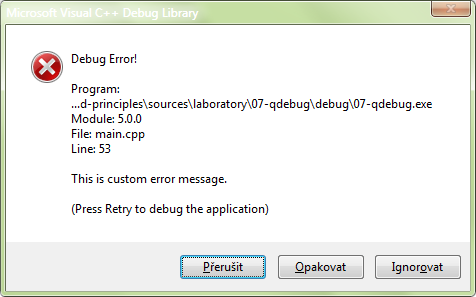
\includegraphics[width=9cm]{graphics/laboratory/11-debugdialog.png}
\caption{Application crash dialog in Windows}\label{figure:errordialog}
\end{figure}

\begin{fdocextra}
Debugging outputs should always be written in English.
\end{fdocextra}

This implementation prints out extra information which is extremely important for debugging. However, you can do whatever you want in your implementation. Storing outputs to database or sending them over network are just some possible enhancements.

The is another (simpler) way of forcing Qt to format console outputs if you want to tweak just format. You may tweak\fdocinlinecode{text}{!}{QT_MESSAGE_PATTERN} build environment variable to display application name or other useful information. Head to the documentation \citep{various:qtdoc} for more information.

\subsection{Working with system environment variables}